\section{Simulations}

\subsection{Constant length pendulum}

In this first part, we will consider the case where \(\alpha=0\) and \(d=0\), that is the length of the pendulum remains constant \(\ell(t)=L\). This corresponds to the situation analysed in \autoref{sec:analytic:constant_length}. Using a small initial angle of \(\theta_0=10^{-10}\) and no initial speed, a convergence study of the final angle and angular speed of the velocity-Verlet method was done. Comparing the final position and angular speed obtained numerically with the analytical results in \autoref{eq:analytic_harmonic_pos} and \autoref{eq:analytic_harmonic_speed}, we obtain an error on the final position and angular velocity. The results in \autoref{fig:numeric_convergence_small_angle} show that the orders of convergence of this method, for these initial conditions, are 4 and 2 for the position and velocity respectively.

\begin{figure}[h]
    \centering
    \begin{subfigure}{0.48\linewidth}
        \centering
        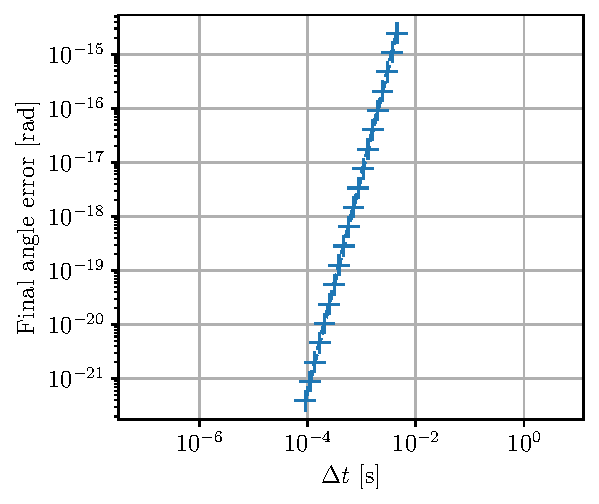
\includegraphics[width=\linewidth]{figures/no_excitation_pos_conv.pdf}
        \caption{Position (angle of pendulum)}
    \end{subfigure}
    \begin{subfigure}{0.48\linewidth}
        \centering
        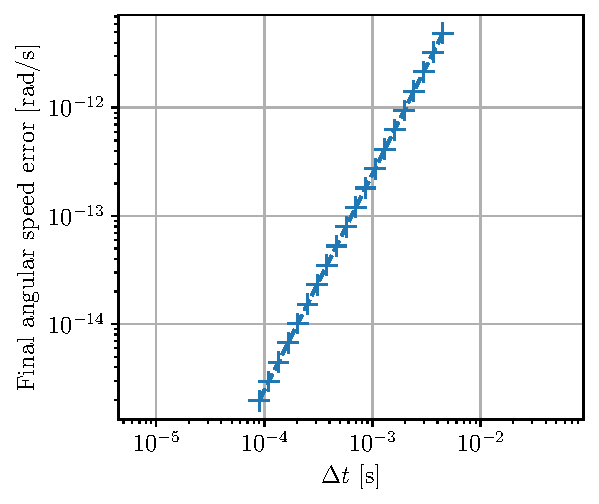
\includegraphics[width=\linewidth]{figures/no_excitation_vel_conv.pdf}
        \caption{Angular velocity}
    \end{subfigure}
    \caption{Numeric convergence of different variables for initial conditions \(\theta_0=10^{-10}\), \mbox{\(\dot\theta_0=0\) \si{\per\second}} and simulated until \(t_\textrm{fin} \approx 2.69\) \si{\second}, corresponding to 3 periods of oscillation}
    \label{fig:numeric_convergence_small_angle}
\end{figure}

Varying the initial angle \(\theta_0\) between \(0\) and \(\pi\) allows us to get larger movements from the pendulum, as shown in \autoref{fig:oscillations_time}. The angular frequency was extracted by looking at the time elapsed between the starting condition and the time it takes for two sign changes in angular speed (otherwise we would be measuring a half-period). Writing that time as \(T\), the period of oscillation, we get the angular frequency \(\Omega = \frac{2\pi}{T}\). The results are shown in \autoref{fig:angular_frequency}. These results are coherent with the physical reality, as a larger angle should correspond to a longer oscillation period than a smaller angle. It is interesting to note that the angular frequency does not change linearly, which is consistent with the results measured in the lab: small angles have less effect than large angles.

\begin{figure}[H]
    \centering
    \begin{subfigure}{0.48\linewidth}
        \centering
        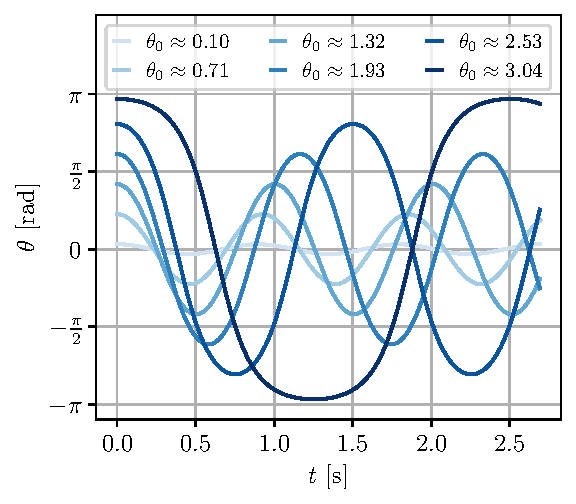
\includegraphics[width=\linewidth]{figures/oscillations_trajectory.pdf}
        \caption{Time evolution}
        \label{fig:oscillations_time}
    \end{subfigure}
    \begin{subfigure}{0.48\linewidth}
        \centering
        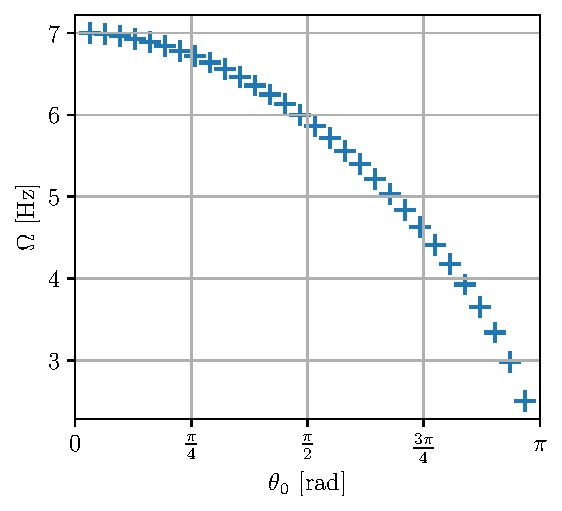
\includegraphics[width=\linewidth]{figures/angular_frequency.pdf}
        \caption{Angular frequency}
        \label{fig:angular_frequency}
    \end{subfigure}
    \caption{Time evolution and angular frequency for multiple starting angles (\(n_\textrm{steps}=10000\))}
\end{figure}


\subsection{Decreasing length pendulum}
The next simulations were run with conditions $\alpha=-0.02$ \si{\meter\per\second} and $d=0$ \si{\meter} and up to $t_\textrm{fin}=0.96L/|\alpha|$ in order to show the behavior of the mass when its rod has a length decreasing almost to 0. First a convergence analysis was done to determine the characteristics of the algorithm when used under these conditions. The various final positions for a given time step $\Delta t$ are shown in \autoref{fig:conv_retract}. Taking the time step squared show the points aligning which indicates that the velocity-Verlet algorithm converged in order 2 for this simulation. This already indicates a greater instability of the system compared to the classical harmonic oscillator.

The first step in studying this system is understanding conceptually how it behaves. As shown in \autoref{fig:retract_time} the oscillations remain low until close to the end of the simulation, corresponding to a very short rod for the pendulum, where they explode.

\begin{wrapfigure}{h}{0.5\linewidth}
    \centering
    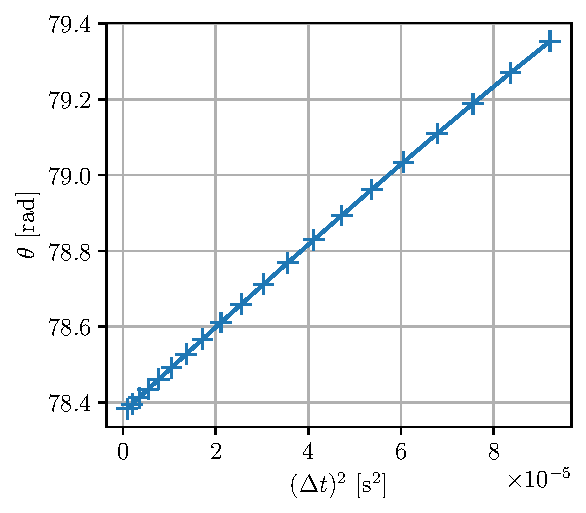
\includegraphics[width=\linewidth]{figures/converg_retraction.pdf}
    \caption{Convergence of the velocity-Verlet algorithm for a pendulum with decreasing length, initial conditions: $\theta_0 = 0.5$, $\dot{\theta}_0 = 0$ \si{\per\second}}
    \label{fig:conv_retract}
\end{wrapfigure}
The values in radians going up to 80 show that in the simulation the pendulum stops oscillating aroung its stable equilibrium and rather does complete rotations around the center $\mathcal{O}$. This is coherent with the fact that it will have not only gained mechanical energy with the work from the tension $T$ but as the rod gets shorter less energy is required to do a complete rotation. The phase space in \autoref{fig:retract_phase} also shows the small oscillations followed by an explosion towards higher values of $\theta$ and $\dot\theta$.

A final physical point of interest is the energy of the system. We want to verify if the algorithm respects the theorem of mechanical energy $\dd E_{mec}/\dd t = P_\mathrm{nonc}$ with $P_\mathrm{nonc}$ the power from non-conservative forces. The \autoref{fig:retract_power} and \autoref{fig:retract_energy} show that this theorem is perfectly verified in this simulation. The \autoref{fig:retract_power} in particular illustrates that the variation of the energy in time, calculated through centered differences, is exactly the power without any visible differences. This can also be illustrated by integrating the power, this is done by summing the small $\dd P = P_\mathrm{nonc} \dd t$, and showing as in \autoref{fig:retract_energy} that substracting it to the energy gives a constant.
\begin{figure}[h]
    \centering
    \begin{subfigure}{0.48\linewidth}
        \centering
        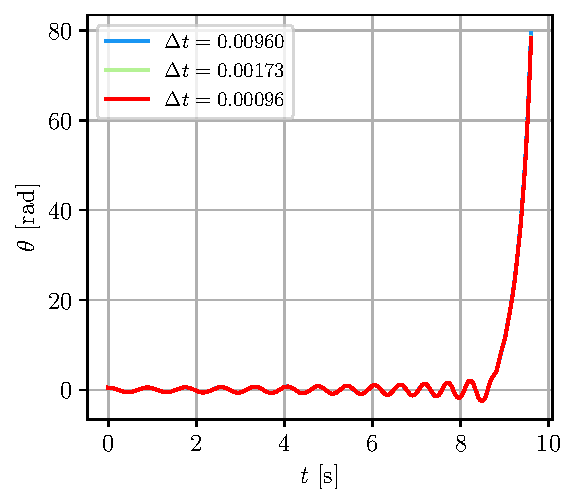
\includegraphics[width=\linewidth]{figures/traj_retraction.pdf}
        \caption{Time evolution}
        \label{fig:retract_time}
    \end{subfigure}
    \begin{subfigure}{0.48\linewidth}
        \centering
        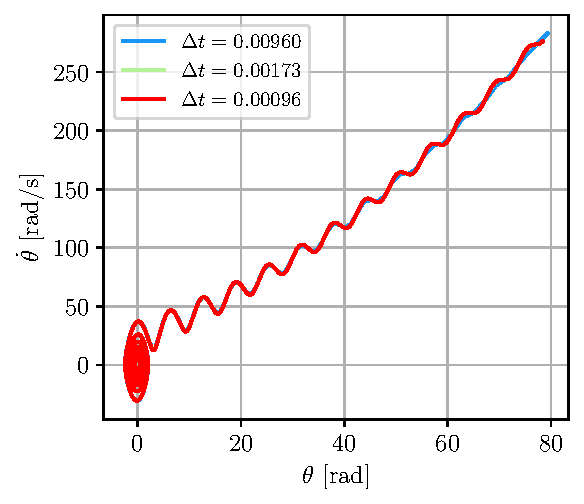
\includegraphics[width=\linewidth]{figures/phase_retraction.pdf}
        \caption{Phase space}
        \label{fig:retract_phase}
    \end{subfigure}
    \caption{Time evolution and phase space of a pendulum with decreasing length during \mbox{$n_\mathrm{steps} = 10000$}; initial conditions: $\theta_0 = 0.5$, $\dot{\theta}_0 = 0$ \si{\per\second}}
\end{figure}

\begin{figure}[H]
    \centering
    \begin{subfigure}{0.48\linewidth}
        \centering
        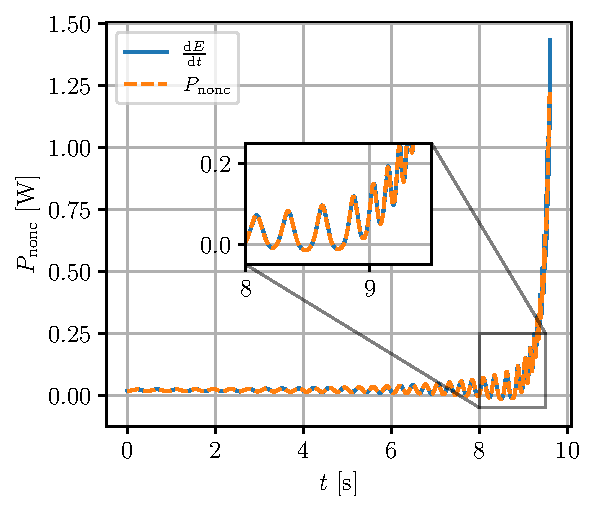
\includegraphics[width=\linewidth]{figures/retract_power.pdf}
        \caption{Power}
        \label{fig:retract_power}
    \end{subfigure}
    \begin{subfigure}{0.48\linewidth}
        \centering
        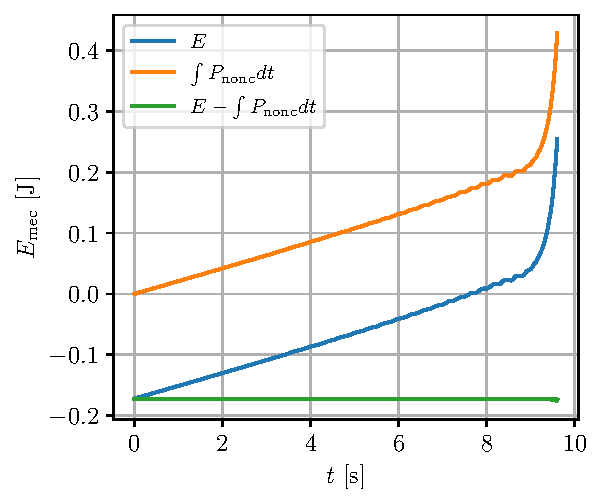
\includegraphics[width=\linewidth]{figures/retract_energy.pdf}
        \caption{Energy}
        \label{fig:retract_energy}
    \end{subfigure}
    \caption{Theorem of mechanical energy for a pendulum with decreasing length; initial conditions: $\theta_0 = 0.5$, $\dot{\theta}_0 = 0$ \si{\per\second}; $n_\textrm{steps}=2000$}
\end{figure}


\subsection{Oscillating length pendulum}
The final case study concerns the conditions $\alpha=0$ \si{\meter\per\second}, $d=0.01$ \si{\meter} and $\omega = 2\omega_0 = 2\sqrt{g/L}$ as calculated in \autoref{sec:analytic:constant_length}.

\begin{wrapfigure}{h}{0.5\linewidth}
    \centering
    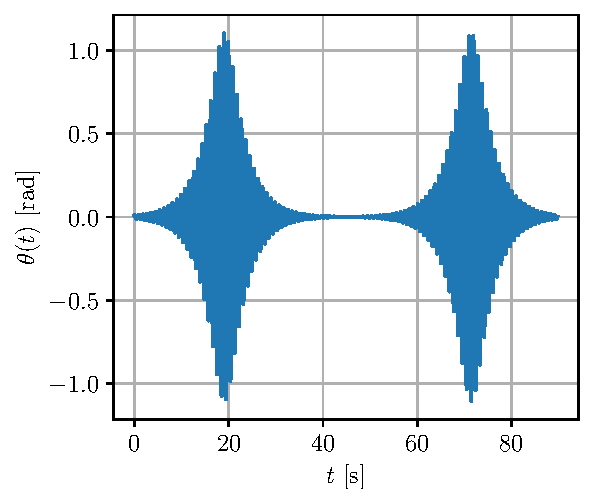
\includegraphics[width=\linewidth]{figures/excitation_smol_traj.pdf}
    \caption{Time evolution of an oscillator excited through varying the length of its rod; initial conditions: \mbox{$\theta_0 = 0.01$}, $\dot{\theta}_0 = 0$ \si{\per\second}; $n_\mathrm{steps} = 1000$ per period of excitation}
    \label{fig:excit_smol}
\end{wrapfigure}
Taking small oscillations, $\theta_0 = 0.01$, we can illustrate the behavior of an excited oscillator as shown in \autoref{fig:excit_smol}. This simulation was run for 200 periods of the oscillation of the length $T_\mathrm{excit} = 2\pi / \omega$. This corresponds numerically to two large oscillations of the amplitude of the smaller oscillations. This behavior indicates that the excitations increase the energy to a maximum, giving larger oscillations, and then start working against it to bring it back to a minimum.

An interesting feature of this new system is the chaotic behavior it can present by taking larger oscillations. We first need to analyse the convergence of our algorithm in this new chaotic system. As can be seen in \autoref{fig:chaos_10_per} the velocity-Verlet algorithm still converges correctly in order 2 for 10 periods of excitation. In this given simulation the final value towards which the algorithm converges in order 2 is $\theta(10T_\mathrm{excit}) = 39.071175$ obtained through a linear fit on the aligned points and evaluated at $\Delta t = 0$. However after too many excitations as shown in \autoref{fig:chaos_20_per}, here 20 periods, with a decreasing $\Delta t$ the final position does not converge to a single value in any polynomial order. It oscillates slightly due to the chaotic nature of the system.
\begin{figure}[h]
    \centering
    \begin{subfigure}{0.48\linewidth}
        \centering
        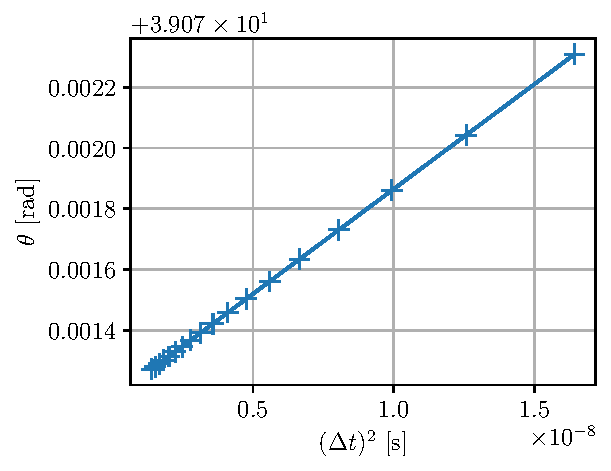
\includegraphics[width=\linewidth]{figures/chaos1_10_periods_conv.pdf}
        \caption{10 periods}
        \label{fig:chaos_10_per}
    \end{subfigure}
    \begin{subfigure}{0.48\linewidth}
        \centering
        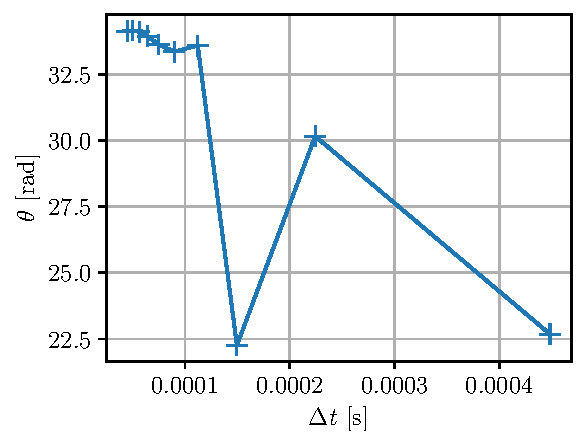
\includegraphics[width=\linewidth]{figures/chaos1_20_periods_conv.pdf}
        \caption{20 periods}
        \label{fig:chaos_20_per}
    \end{subfigure}
    \caption{Convergence of the velocity-Verlet algorithm for a chaotic system and different numbers of periods of excitation; initial conditions: $\theta_0 = 0$, $\dot{\theta}_0 = 15$ \si{\per\second}}
\end{figure}

To further illustrate the chaos in this system we can show the strong dependence on initial conditions. The distance $\delta$ represented in \autoref{fig:lyapounov} was calculated with the formula:
\begin{equation}
    \delta(t) = \sqrt{\omega_0^2(\theta_1(t) - \theta_2(t))^2 + (\dot\theta_1(t) - \dot\theta_2(t))^2}
\end{equation}
It represents a type of distance between two trajectories during 40 periods of excitation, $\theta_1$ and $\theta_2$, corresponding respectively to the initial conditions $\theta_{0,1} = 0$, $\dot\theta_{0,1} = 15$ \si{\per\second} and $\theta_{0,2} = 10^{-6}$, $\dot\theta_{0,2} = 15$ \si{\per\second}. These two very close initial conditions give diverging trajectories as illustrated by the growth of the distance $\delta$. This represents an exponential growth of the divergence of the trajectories. This exponential has the exponent of Lyapounov: $\lambda \approx 0.76$. This allows to characterise the chaos of this system by knowing the rate of growth of the divergence of trajectories with similar starting conditions.

\begin{figure}[H]
    \centering
    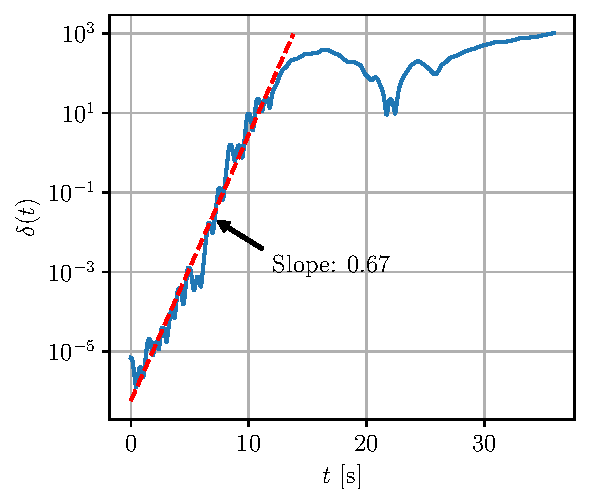
\includegraphics[width=0.6\linewidth]{figures/lyapounov.pdf}
    \caption{Distance in the phase space between two chaotic trajectories for an oscillator with varying length, indication of the Lyapounov exponent, $n_\mathrm{steps} = 10000$ per period of excitation}
    \label{fig:lyapounov}
\end{figure}



\subsection{Poincaré map}
The same chaotic system can be sampled more clearly through a Poincaré map. To achieve this we run the simulation with a set number of steps $n_\mathrm{steps} = 1000$ per period of excitation and we sample the phase space at every period. The \autoref{fig:poincaré} shows the results for 9 different given initial conditions and 30 000 periods. We see that for certain small enough values of the initial energy we have a simple poincaré map representing a non-chaotic system. This is illustrated with the conditions going up to $\theta_0=0$, $\dot\theta_0=10$ \si{\per\second}. For these conditions the system will show a behavior similar to the one obtained in \autoref{fig:excit_smol}. A difference that can be noted between these non-chaotic systems is that the one with $\theta_0 > 0$, $\dot\theta_0 > 0$ has a jump between two symetrical parts of the system. This represents a certain phase with the excitations such that it never reaches small values of $\theta$ or $\dot\theta$ at the end of an excitation period. Some other non-chaotic conditions do not approach the origin $(\theta = 0, \dot\theta = 0)$ and they represent oscillations for which the tension does not produce enough work against to bring them to very small energies.

We can observe two boundary conditions, still on \autoref{fig:poincaré}, at $\dot\theta_0=11.88$ \si{\per\second} and \mbox{$\dot\theta_0=12.13$ \si{\per\second}}. These conditions are also non-chaotic. The first one gives small "islands" representing a certain phase with the excitations. The second one is the closest value found to the limit before reaching chaotic systems. Any test simulation run with greater initial energies than for this one led to chaotic systems.

Above this treshold of initial energy the system becomes chaotic and samples the same shape shown by the two different chaotic systems in the \autoref{fig:poincaré}. This shows that the chaos is not pure randomness but instead it samples a certain precise part of the phase space in a seemingly random way, that is underneath deterministic according to classical mechanics. A final simulation with a very large $\dot\theta_0$, here 20 \si{\per\second}, was run and it shows that at some point very fast rotations do not leave enough space for the oscillations of the length to play a big part in the system. The system simply rotates very fast around $\mathcal{O}$ and is not chaotic anymore.
\begin{figure}[H]
    \centering
    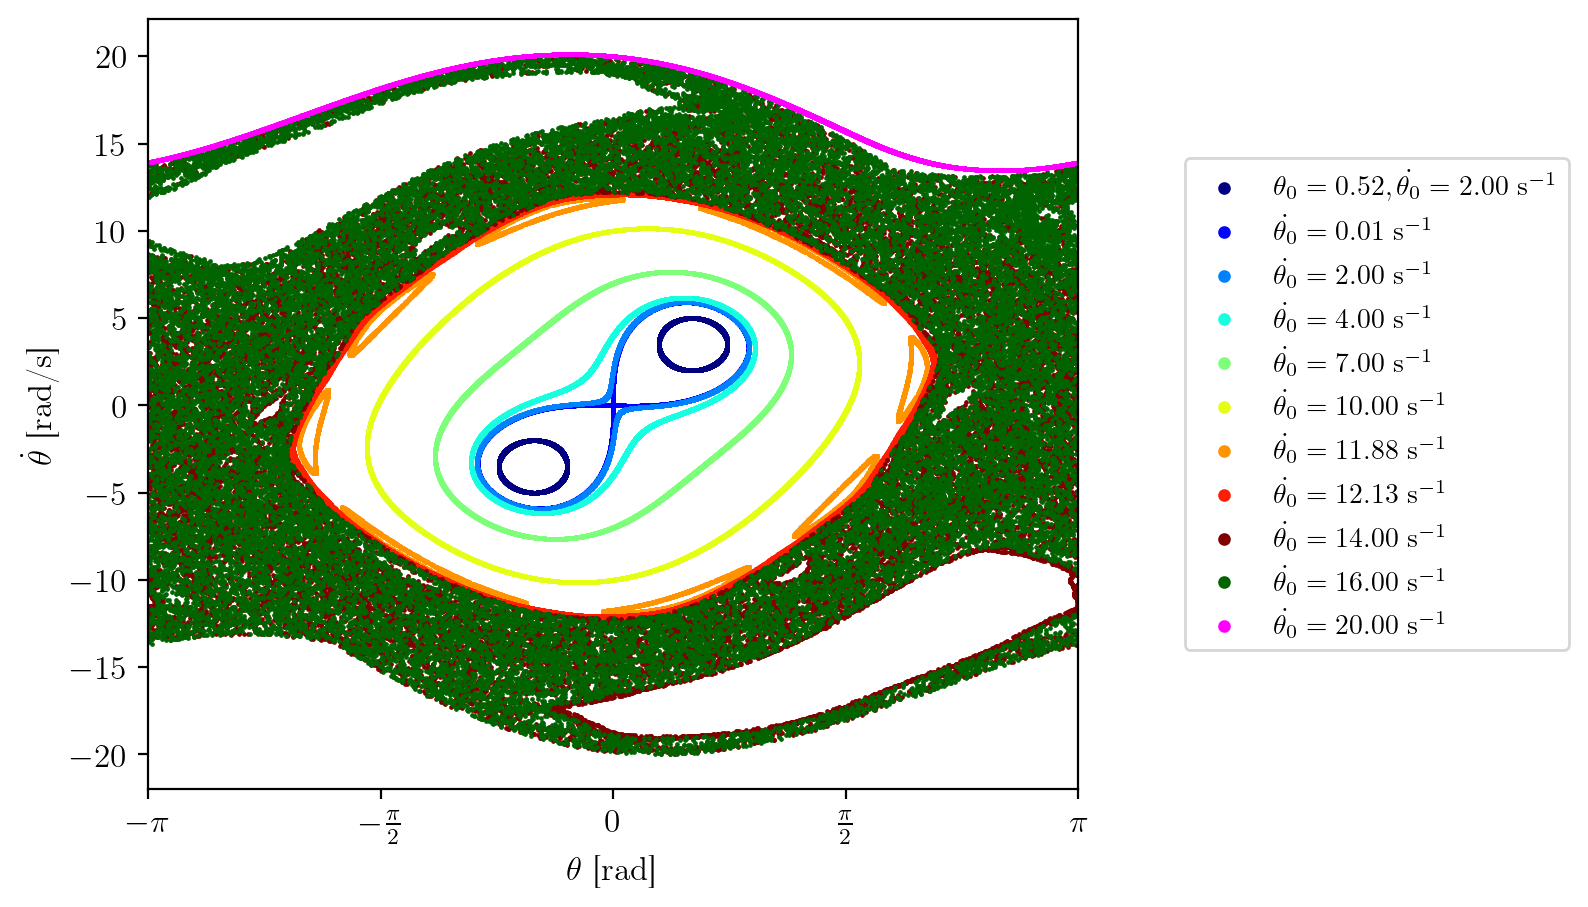
\includegraphics[width=\linewidth]{figures/poincare_overkill.png}
    \caption{Poincaré map of a chaotic system, a pendulum with varying length, for various initial conditions, \(\theta_0=0\) unless said otherwise (\(n_\textrm{steps}=1000\), \(N=30 000\) periods of excitation)}
    \label{fig:poincaré}
\end{figure}





